\section{Multiple Groups Case}\label{app:multi-group}

\begin{figure}[t]
	\centering
	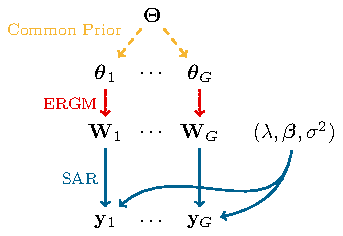
\includegraphics[scale=1]{figures-tikz/ergm-hierarchical.pdf}
	\caption{\acrshort{sar} with multiple groups and \acrshort{ergm} prior.}
	\label{fig:sar-ergm-multi-group}
\end{figure}

\begin{algorithm}[t]
	\centering
	\begin{algorithmic}[1]
		\STATE Initialize $(\lambda^{(0)}, \{\WW^{(0)}_{g}\}, \bbeta^{(0)}, \sigma^{2(0)}, \{\ttheta_{g}^{(0)}\})$
		\FOR[ Run Gibbs Sampling for length $T$ ]{ $t=1$ \TO $T$ }
		\STATE $\lambda^{(t)}$ $\gets$ sample from conditional posterior $\pr(\lambda\given\{\yy_{g}\},\{\WW_{g}^{(t-1)}\},\bbeta^{(t-1)},\sigma^{2(t-1)})$ with \acrshort{gg} algorithm
		\STATE $\bbeta^{(t)}$  $\gets$ sample from $\pr(\bbeta\given\{\yy_{g}\},\lambda^{(t)},\{\WW_{g}^{(t-1)}\},\sigma^{2(t-1)})$ directly
		\STATE $\sigma^{2(t)}$ $\gets$ sample from $\pr(\sigma^{2}\given\{\yy_{g}\},\lambda^{(t)},\{\WW_{g}^{(t-1)}\},\bbeta^{(t)})$ directly
		\FOR { $g'=1$ \TO $G$ }
		\STATE $\WW_{g'}^{(t)}$ $\gets$ sample from
		$\pr(\WW_{g'}\given\yy_{g'},\lambda^{(t)},\bbeta^{(t)},\sigma^{2(t)},\ttheta_{g'}^{(t-1)})$
		with \acrshort{hmc} algorithm
		\STATE $\ttheta_{g'}^{(t)}$ $\gets$ sample from conditional posterior $\pr(\ttheta\given\WW_{g}^{(t)})$ with \acrshort{ex} algorithm
		\ENDFOR
		\ENDFOR
	\end{algorithmic}
	\caption{Gibbs Sampling for Hierarchical Bayes Specification.}
	\label{alg:gibbs}
\end{algorithm}

In many applications,
we have multiple groups of actors on which we believe network structures sharing common characteristics exist.
For example, we might observe similar friendship network characteristics in different classrooms.

To incorporate these kinds of scenarios in our model,
we introduce group subscript $g=1,...,G$.
Explicitly, we now have a subscripted variation of \eqref{eq:likelihood} as
\begin{align*}
	f(\yy_{g}\given\pphi_{g})
	=
	(2\pi)^{-N_{g}/2}
	\det(\VV_{\yy}(\pphi_{g}))^{-1/2}
	\exp\left( -\frac12 \norm[ \VV_{\yy}(\pphi_{g}) ]{ \yy_{g}-\yhat_{g}(\pphi_{g}) }^2 \right)
\end{align*}
where $N_{g}$ is the size of group $g$,
$\pphi_{g}$ is $\{\lambda,\WW_{g},\beta,\sigma^2\}$,
$\VV_{\yy}(\pphi_{g})$ is the variance
$\sigma^2\MM(\pphi_{g})\inv\MM(\pphi_{g})\invT$
and $\yhat_{g}(\pphi_{g})$ is the reduced-form
$\MM(\pphi_{g})\inv\HH_{g}\bbeta.$
Thus, we have the likelihood of observing the entire data $\{\yy_{g}\}$ as
\begin{align*}
	\pr(\{\yy_{g}\}\given\lambda,\{\WW_{g}\},\bbeta,\sigma^{2})
	=
	\prod_{g} \pr(\yy_{g}\given\pphi_{g}),
\end{align*}
assuming independence between groups.

Now we have the hierarchical Bayesian model as
\begin{align*}
	\begin{cases}
		\lambda                   &\sim \Uniform(\ubar{\lambda},\bar{\lambda}), \\
		\bbeta                    &\sim \Normal(0,\VV_{\bbeta}), \\
		\sigma^2                  &\sim \InverseGamma(a_{\sigma^2},b_{\sigma^2}), \\
		\ttheta                   &\sim \Normal(0,\VV_{\ttheta}), \\
		\pr(\WW_{g}\given\ttheta) &\propto \exp(\ss(\WW_{g})\T\ttheta), \\
		\yy_{g}\given\lambda,\WW_{g},\bbeta,\sigma^2 &\sim \Normal(\yhat_{g}(\pphi_{g}),\VV_{\yy}(\pphi_{g})).
	\end{cases}
\end{align*}
This hierarchical model is represented as a \acrshort{dag} in \autoref{fig:sar-ergm-multi-group}.
The corresponding posterior distributions are quite similar those described in \autoref{sec:prior-sar} and \autoref{sec:prior-ergm},
the detailed derivations are presented in \autoref{app:derivation-of-posteriors}.

The outline of the Gibbs sampling procedure is presented in \autoref{alg:gibbs}.
We will have to adjust the \acrshort{ergm} model by group size, as suggested in \cite{krivitsky-handcock-morris-2011}.

\subsection{Simulation: Mock 1}

\begin{table}[t]
	\centering
	\begin{tabular}{l|c}
		\toprule
		Parameter & Value \\
		\midrule
		$\lambda$ & 0.05 \\
		$(\bbeta_1\T,\bbeta_2\T)$ & $(1,0.5)$ \\
		$\sigma^2$ & $1$ \\
		$\ttheta_{\text{\Verb"edges"}}$  & $-2$ \\
		$\ttheta_{\text{\Verb"mutual"}}$ & $2$ \\
		\bottomrule
	\end{tabular}
	\caption{Simulation 1 True Parameters}
	\label{tab:simulation-1-params}
\end{table}

In this simulation, we consider a data set of $G=10$ groups.
For each group $g\in\{1,...,G\}$, the network is generated from an \acrshort{ergm} with two sufficient statistics:
number of edges and number of mutual links.
\footnote{This specification corresponds to the \Verb"ergm.term"'s \Verb"edges" and \Verb"mutual" from the R package \Verb"ergm".}
Then, we observe $\{\yy_{g},\XX_{g}\}$ according to the \acrshort{sar} \acrshort{dgp}
\begin{align*}
	\yy_{g} = \lambda \WW_{g} \yy_{g} + \XX_{g} \bbeta_{1} + \WW_{g} \XX_{g} \bbeta_{2} + \uu_{g}
\end{align*}
where $\uu_{g}$ follows $\Normal(0,\sigma^2)$ and $\XX_{g}$ has one column (thus $\bbeta_1$ and $\bbeta_2$ are both scalars).
The group sizes are consecutive integers from $15$ to $24$.
The values of the true parameters are shown in \autoref{tab:simulation-1-params}.

